\documentclass{article}
\usepackage{geometry}
 \geometry{
 letterpaper,
 left=1in,
 right=1in,
 top=1in,
 bottom=1in,
 }
\usepackage[utf8]{inputenc}
\usepackage[T1]{fontenc}

\usepackage{amsmath,float}
\floatplacement{figure}{H}
\usepackage{hyperref}
\usepackage{tikz,pgfplots}
\pgfplotsset{compat=1.12}

\graphicspath{{./images/}}
%% Commande supplémentaire

% semi-norm of a vector
\newcommand{\snorm}[1]{\left| #1 \right|}
% norm of a vector
\newcommand{\norm}[1]{\left\| #1 \right\|}
% degree symbol
\newcommand{\degree}[0]{^\circ} 
% rename builtin command \v{} to \vaccent{}
\let\vaccent=\v 
% for vectors
\renewcommand{\v}[1]{\ensuremath{\mathbf{#1}}} 
% for vectors of Greek letters
\newcommand{\gv}[1]{\ensuremath{\mbox{\boldmath$ #1 $}}} 
% for unit vector
\newcommand{\uv}[1]{\ensuremath{\mathbf{\hat{#1}}}}	
% for tensors
%\newcommand{\tn}[1]{\ensuremath{\pmb{\mathsf{#1}}}} 
% for tensors of Greek letters
\newcommand{\tn}[1]{\ensuremath{\mbox{\boldmath$\mathsf{#1}$}}} 
% for absolute value
\newcommand{\abs}[1]{\left| #1 \right|}	
% for average
\newcommand{\avg}[1]{\left< #1 \right>} 
% rename builtin command \d{} to \underdot{}
\let\underdot=\d 
% for derivatives
\renewcommand{\d}[2]{\frac{d #1}{d #2}} 
% for double derivatives
\newcommand{\dd}[2]{\frac{d^2 #1}{d #2^2}} 
% for partial derivatives
\newcommand{\pd}[2]{\frac{\partial #1}{\partial #2}}
% for double partial derivatives
\newcommand{\pdd}[2]{\frac{\partial^2 #1}{\partial #2^2}} 
% for crossed double partial derivatives
\newcommand{\pdx}[3]{\frac{\partial^2 #1}{\partial #2 \partial #3}} 
% for thermodynamic partial derivatives
\newcommand{\pdc}[3]{\left( \frac{\partial #1}{\partial #2} \right)_{#3}} 
% for Dirac bras
\newcommand{\ket}[1]{\left| #1 \right>} 
% for Dirac kets
\newcommand{\bra}[1]{\left< #1 \right|} 
% for Dirac brackets
\newcommand{\braket}[2]{\left< #1 \vphantom{#2} \right| \left. #2 \vphantom{#1} \right>} 
% for Dirac matrix elements
\newcommand{\matrixel}[3]{\left< #1 \vphantom{#2#3} \right| #2 \left| #3 \vphantom{#1#2} \right>} 
% for gradient
\newcommand{\grad}[1]{\gv{\nabla} #1}
% rename builtin command \div to \divsymb
\let\divsymb=\div 
% for divergence
\renewcommand{\div}[1]{\gv{\nabla} \cdot #1} 
% for curl
\newcommand{\curl}[1]{\gv{\nabla} \times #1} 
% for laplacian
\newcommand{\lap}[1]{\gv{\nabla}^2 #1}
% Math text
\newcommand{\mt}[1]{\mathrm{#1}} 
% Overline
\newcommand{\ol}[1]{\overline{#1}}
% Partial derivative with dfrac
\newcommand{\dpd}[2]{\dfrac{\partial #1}{\partial #2}}
% Scientific notation
\providecommand{\e}[1]{\ensuremath{\times 10^{#1}}}
% Symbole degré
\renewcommand{\deg}{$^{\circ}\;$}

% text style
%
\newcommand{\Ae}{\text{\normalshape a.e.}}
% c'est-à-dire
\newcommand{\ie}{\textit{i.e.}\ }
% e.g. - par exemple
\newcommand{\eg}{\textit{e.g.}\ }
\newcommand{\strong}{\text{\normalshape -strong}}
\newcommand{\weak}{\text{\normalshape -weak}}
\newcommand{\loc}{\text{\normalshape loc}}
\newcommand{\ad}{\text{\normalshape ad}}
% Symbole degré
\renewcommand{\deg}{$^{\circ}\;$}
% Accronymes
\newcommand{\PIV}{\textit{PIV}\ }

% Space operator
\newcommand{\Def}{\overset{\text{\textup{def}}}{=}}
\newcommand{\R}{\operatorname{\mathbb R}}
\newcommand{\Rn}{\operatorname{{\mathbb R}^N}}
\newcommand{\RK}{\operatorname{{\mathbb R}^K}}
\newcommand{\N}{\operatorname{\mathbb N}}
\newcommand{\Z}{\operatorname{\mathbb Z}}
\newcommand{\ON}{\operatorname{\text{\textup{O(N)}}}}
\newcommand{\opt}{\mathrm{opt}}

% Matrix operator
\newcommand{\transp}{\:{}^*\,\negmedspace}
\newcommand{\trans}{\:{}^* \negmedspace}
\newcommand{\transm}{\:{}^* \!\negmedspace}
\newcommand{\tran}{{}^* \negmedspace}

% Environnement pour les Théorème, lemmes et remarques
\newtheorem{theoreme}{Th\'{e}or\`{e}me}
\newtheorem{lemme}{Lemme}
\newtheorem{remarque}{Remarque}
\newtheorem{prop}{Proposition}
\newtheorem{hypo}{Hypoth\`{e}se}
\newtheorem{dfn}{D\'{e}finition}

% Variables
\newcommand{\constant}[1]{\mathit{#1}}
\renewcommand\Re{\constant{Re}}  % Reynolds number
\newcommand\Pe{\constant{Pe}}  % Peclet number
\newcommand\Nu{\constant{Nu}}  % Nusselt number
\newcommand\Sh{\constant{Sh}}  % Sherwood number
\newcommand\Sc{\constant{Sc}}  % Schmidt number
\renewcommand\Pr{\constant{Pr}}  % Prandlt number
% Trucs de chimie
\newcommand\el{\mathrm{e^-}}
\newcommand*\chem[1]{\ensuremath{\mathrm{#1}}}

% used tikz libraries
\usetikzlibrary{patterns}
\usetikzlibrary{arrows}
\usetikzlibrary{calc}
\usetikzlibrary{intersections}
\usetikzlibrary{trees}
\usetikzlibrary{positioning}
\usetikzlibrary{arrows}
\usetikzlibrary{chains}
\usetikzlibrary{decorations.shapes}
\usetikzlibrary{decorations.pathreplacing}
\usetikzlibrary{decorations.pathmorphing}
\usetikzlibrary{decorations.markings}
\usetikzlibrary{shapes}
\usetikzlibrary{matrix}

\begin{document}

%=== SCHÉMA GLOBAL MÉTHODE INVERSE ===%
\begin{figure}[!ht]
\centering
\tikzset{
	My Line Style/.style={smooth, ultra thick, samples=400},
	punktchain/.style={
		rectangle, 
		rounded corners, 
		% fill=black!10,
		draw=black, very thick,
		text width=20em, 
		minimum height=3em, 
		text centered, 
		on chain},
	line/.style={draw, thick, <-},
	punktchain2/.style={
		rectangle, 
		rounded corners, 
		% fill=black!10,
		draw=black, very thick,
		text width=15em, 
		minimum height=3em, 
		text centered, 
		on chain},
	every join/.style={->, thick,shorten >=1pt,>=stealth},
	decorate sep/.style 2 args=
	{decorate,decoration={shape backgrounds,shape=circle,shape size=#1,shape sep=#2}}
}

\begin{tikzpicture}
[node distance=.8cm,
start chain=going below,]
\draw (0,1.3) node{};
\draw (0,-15.5) node{};
\node[punktchain,dashed] (0) {Mesures \mbox{expérimentales} du courant de diffusion $I(t)$ et calcul du transfert de masse \vspace{-0.3cm}
	\begin{align*} 
	K(t)=\dfrac{I(t)}{nFAC_0} \to Sh_{exp}(t^*) = \dfrac{K(t^*)l}{D}
	\end{align*}
};
\node[punktchain] (1) {1. Résolution de XYZ avec $\hat{S}^*(t^*_k)$, une bonne approximation de $S^*(t^*_k)$};
%     \draw[decorate sep={0.8mm}{1.2mm},fill] (0) -- (1);
\node[punktchain, join] (2) {2. Évaluation de $\hat{\Sh}(t^*_k)$ en intégrant le transfert de masse à la sonde, d'après XYZ};
\node[punktchain, join] (3) {3. Calcul de $\partial\hat{Sh}(t^*_k)/\partial{S^*}$ (c.f. sect. XYZ) et correction de $\hat{S}^*(t^*_k)$: \vspace{-0.4cm}
	\begin{align*}
	S^*_i(t^*_k) &= \hat{S}^*(t^*_k) + dS
	\end{align*} };
\node[punktchain, join] (4) {4. Résolution de XYZ0 avec $S^*_i(t^*_k)$, puis évaluation de $Sh_i(t^*_k)$ avec XYZ};
\node[punktchain, join] (5) {5. Vérification de la convergence de $Sh_i(t^*_k)$ \vspace{-0.3cm}
	\begin{align*}
	|Sh_i(t^*_k) - Sh_{exp}(t^*_k)| < \epsilon \;?
	\end{align*} 
};
\begin{scope}[start branch]
	\node[punktchain2, on chain=going right] (6) { \vspace{-0.5cm}
		\begin{align*} 
		6. \;\; \hat{S}^*(t^*_k) &= S^*_i(t^*_k) \\
		i &= i+1
		\end{align*}
	};
\end{scope}
\draw[->, thick,>=stealth] (5) -- node [above] {non} (6);
\draw[dashed,->, ultra thick,>=stealth] (6.north) |- (1.east);
\node[punktchain] (7) { \vspace{-0.5cm}
	\begin{align*}
	7.\;\; S^*_{inv}(t^*_k) = S^*_i(t^*_k) &\quad\;  Sh_{inv}(t^*_k) = Sh_i(t^*_k)\\
	\hat{S}^*(t^*_{k+1}) &= S^*_i(t^*_k) \\
	k &= k+1
	\end{align*}
};
\draw[->, thick,>=stealth] (5) -- node [left] {oui} (7);
\node[on chain=going left] (caca) {};
\draw[dashed,->, ultra thick,>=stealth] (7.west) -- (caca.center)  |- (1);
\end{tikzpicture}
\end{figure}


%=== flowchart inverse method ===%
\begin{figure}[!ht]
\centering
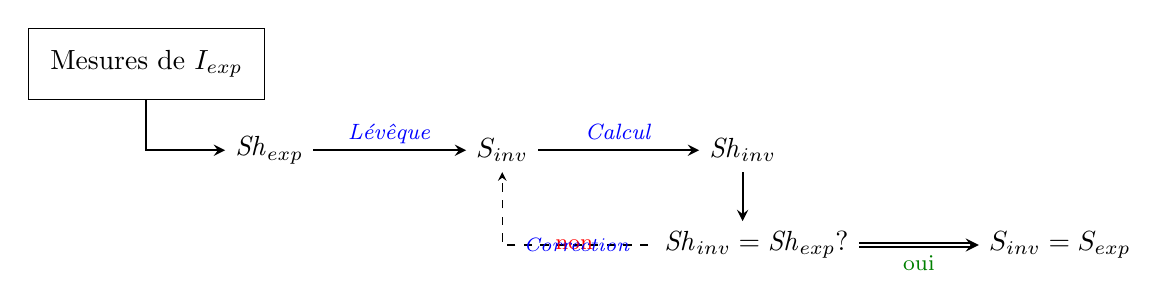
\begin{tikzpicture}
\draw rectangle(3,0.9) node[pos=.5] {Mesures de $I_{exp}$};
\draw[thick,->,>=stealth] (1.5,0) |- +(1,-0.65) node[right] (a){$\Sh_{exp}$};%(a);
\draw[thick,->,>=stealth] (a) -- node[above=-0.05cm]{\color{blue}\footnotesize \textit{Lévêque}} +(2.5,0) node[right](b){$S_{inv}$};
\draw[thick,->,>=stealth] (b) --  node[above]{\color{blue}\footnotesize \textit{Calcul}} +(2.5,0) node[right](b1){$\Sh_{inv}$};
\draw[thick,->,>=stealth] (b1) -- +(0,-0.9) node[below](c) {$\quad\Sh_{inv} = \Sh_{exp}$?};
\draw[->,dashed,>=stealth] ($(c)-(1.2,0)$) -| node[below=0.3cm, right=0.55cm] {\footnotesize \color{red} non} node[above=0.25cm, right=0.15cm,] {\color{blue}\scriptsize \textit{Correction}} (b);
\draw[->,thick,double,>=stealth] (c) -- node[below]{\footnotesize \color{green!50!black} oui} +(3,0) node[right]{$S_{inv}=S_{exp}$};
\end{tikzpicture}
\end{figure}

\end{document}